% vim: set spell spelllang=en tw=100 et sw=4 sts=4 foldmethod=marker foldmarker={{{,}}} :

\documentclass{beamer}

\usepackage{tikz}
\usepackage{xcolor}
\usepackage{complexity}
\usepackage{hyperref}
\usepackage{gnuplot-lua-tikz}
\usepackage[vlined]{algorithm2e} % algorithms

\usetikzlibrary{shapes, arrows, shadows, calc, positioning, fit}
\usetikzlibrary{decorations.pathreplacing, decorations.pathmorphing, shapes.misc}
\usetikzlibrary{tikzmark}

\colorlet{screenverylightgrey}{black!2!white}
\colorlet{screengrey}{black!30!white}

\definecolor{uofgblue}{rgb}{0, 0.321569, 0.533333}
\colorlet{uofgblue20}{uofgblue!20!white}
\colorlet{uofgblue40}{uofgblue!40!white}
\colorlet{uofgblue60}{uofgblue!60!white}
\colorlet{uofgblue80}{uofgblue!80!white}

\definecolor{uofgstone}{rgb}{0.498039, 0.454902, 0.403922}

\definecolor{uofgtdarkgreen}{rgb}{0.380392, 0.564706, 0.501961}
\definecolor{uofgtlightgreen}{rgb}{0.615686, 0.788235, 0.729412}
\definecolor{uofgtyellow}{rgb}{0.85098, 0.827451, 0.643137}
\definecolor{uofgtorange}{rgb}{0.784314, 0.694118, 0.545098}

% make gnuplot graphs use our preferred choice of colours.
\colorlet{gp lt color 0}{uofgblue40}
\colorlet{gp lt color 1}{uofgblue60}
\colorlet{gp lt color 2}{uofgtlightgreen!50!white}
\colorlet{gp lt color 3}{uofgtlightgreen}
\colorlet{gp lt color 4}{uofgblue}
\colorlet{gp lt color 5}{black}
\colorlet{gp lt color 6}{uofgtdarkgreen}
\colorlet{gp lt color 7}{uofgtorange}

% {{{ theme things
\useoutertheme[footline=authortitle]{miniframes}
\useinnertheme{rectangles}

\setbeamerfont{block title}{size={}}
\setbeamercolor*{structure}{fg=uofgblue}
\setbeamercolor*{palette primary}{use=structure,fg=black,bg=white}
\setbeamercolor*{palette secondary}{use=structure,fg=black,bg=uofgblue40}
\setbeamercolor*{palette tertiary}{use=structure,fg=white,bg=uofgblue}
\setbeamercolor*{palette quaternary}{fg=white,bg=black}

\setbeamercolor*{titlelike}{parent=palette primary}

\beamertemplatenavigationsymbolsempty

\setbeamertemplate{title page}
{
    \vbox{}
    \vspace*{0.5cm}
    \begin{centering}
        {\usebeamerfont{title}\inserttitle\par}
        \vskip0.5cm\par
        \begin{beamercolorbox}[sep=8pt,center]{author}
            \usebeamerfont{author}\insertauthor
        \end{beamercolorbox}
        {\usebeamercolor[fg]{titlegraphic}\inserttitlegraphic\par}
    \end{centering}
    \vfill

    \begin{tikzpicture}[remember picture, overlay]
        \node at (current page.north west) {\begin{tikzpicture}[remember picture, overlay]\fill
        [fill=uofgblue, anchor=north west] (0, 0) rectangle (\paperwidth, -1.5cm);\end{tikzpicture}};
        \node [anchor=north west, shift={(0.2cm,-0.2cm)}] at (current page.north west) {\includegraphics*[keepaspectratio=true,scale=0.5]{UoG_keyline.eps}};
    \end{tikzpicture}
}

\newcommand{\frameofframes}{/}
\newcommand{\setframeofframes}[1]{\renewcommand{\frameofframes}{#1}}

\makeatletter
\setbeamertemplate{footline}
{%
    \begin{beamercolorbox}[colsep=1.5pt]{upper separation line foot}
    \end{beamercolorbox}
    \begin{beamercolorbox}[ht=2.5ex,dp=1.125ex,%
        leftskip=.3cm,rightskip=.3cm plus1fil]{author in head/foot}%
        \leavevmode{\usebeamerfont{author in head/foot}\insertshortauthor}%
        \hfill%
        {\usebeamerfont{institute in head/foot}\usebeamercolor[fg]{institute in head/foot}\insertshortinstitute}%
    \end{beamercolorbox}%
    \begin{beamercolorbox}[ht=2.5ex,dp=1.125ex,%
        leftskip=.3cm,rightskip=.3cm plus1fil]{title in head/foot}%
        {\usebeamerfont{title in head/foot}\insertshorttitle}%
        \hfill%
        {\usebeamerfont{frame number}\usebeamercolor[fg]{frame number}\insertframenumber~\frameofframes~\inserttotalframenumber}
    \end{beamercolorbox}%
    \begin{beamercolorbox}[colsep=1.5pt]{lower separation line foot}
    \end{beamercolorbox}
}
\makeatother

% }}}

\title{Search and Discrepancies}
\author[Ciaran McCreesh]{\textcolor{uofgblue}{Ciaran McCreesh}}

\begin{document}

{
    \usebackgroundtemplate{\includegraphics*[keepaspectratio=true, height=\paperheight]{background.jpg}}
    \begin{frame}[plain]
        \titlepage
    \end{frame}
}

\begin{frame}{This Week's Lectures}
    \begin{columns}
        \column{.5\textwidth}
        \begin{itemize}
            \item Search and Discrepancies
            \item Parallel CP
            \item Parallel Search
        \end{itemize}
        \column{.5\textwidth}
        \centering\includegraphics*[keepaspectratio=true,scale=0.5]{search-but-not-as-we-know-it.jpg}
        \begin{center}``It's search, Jim, but not\\as we know it.''\end{center}
    \end{columns}
\end{frame}

\begin{frame}{Maintaining Arc Consistency (MAC)}
    \begin{itemize}
        \item Achieve (generalised) arc consistency (AC3, etc).
        \item If we have a domain wipeout, backtrack.
        \item If all domains have one value, we're done.
        \item Pick a variable (using a heuristic) with more than one value, then branch:
            \begin{itemize}
                \item Try giving it one of its possible values (using a heuristic), and recurse.
                \item If that failed, reject that value, pick a new value, and try again.
                \item If we run out of values, backtrack.
            \end{itemize}
    \end{itemize}
\end{frame}

\begin{frame}{Search as a Tree}

    \centering
    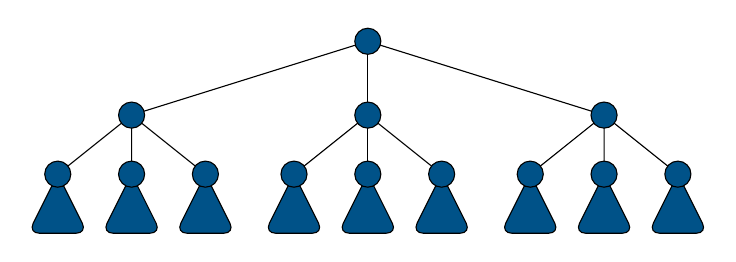
\begin{tikzpicture}[scale=0.75]%{{{
        \coordinate (R);

        \coordinate (N) at (R);

        \coordinate (N1) at ($(N) + (-4, -1.25)$);
        \coordinate (N2) at ($(N) + ( 0, -1.25)$);
        \coordinate (N3) at ($(N) + ( 4, -1.25)$);

        \foreach \na in {1, ..., 3}{
            \coordinate (N\na 1) at ($(N\na) + (-1.25, -1)$);
            \coordinate (N\na 2) at ($(N\na) + ( 0,    -1)$);
            \coordinate (N\na 3) at ($(N\na) + ( 1.25, -1)$);

            \foreach \nb in {1, ..., 3}{
                \coordinate (N\na\nb t1) at ($(N\na\nb) + (-0.5, -1)$);
                \coordinate (N\na\nb t2) at ($(N\na\nb) + ( 0.5, -1)$);
            }
        }

        \foreach \na in {1, ..., 3}{
            \draw (N) -- (N\na);
            \foreach \nb in {1, ..., 3}{
                \draw (N\na) -- (N\na\nb);
            }
        }

        \tikzstyle{t} = [draw, fill, fill=uofgblue, rounded corners];
        \foreach \na in {1, ..., 3}{
            \foreach \nb in {1, ..., 3}{
                \draw [t] (N\na\nb) -- (N\na\nb t1) -- (N\na\nb t2) -- cycle;
            }
        }

        \tikzstyle{c} = [draw, circle, fill, fill=uofgblue];
        \node [c] at (N) { };

        \foreach \na in {1, ..., 3}{
            \node [c] at (N\na) { };

            \foreach \nb in {1, ..., 3}{
                \node [c] at (N\na\nb) { };
            }
        }
    \end{tikzpicture}%}}}

    \vspace{1em}

    \begin{itemize}
        \item Circles are recursive calls, triangles are `big' subproblems.
        \item MAC is like Depth-First Search (DFS).
        \item Heuristics determine the `shape' of the tree.
    \end{itemize}
\end{frame}

\begin{frame}{Heuristics and Discrepancies}

    \begin{itemize}
        \item If our heuristics are perfect, and an instance is satisfiable, we walk straight to a
            solution by going left at every level.
        \item If an instance is unsatisfiable, perfect heuristics would give the smallest possible
            search tree.
        \item But heuristics aren't perfect\ldots
        \item We call going against a heuristic choice a ``discrepancy''.
    \end{itemize}

\end{frame}

\begin{frame}{Two Claims Regarding Heuristics and Search}

    \begin{enumerate}
        \item The total number of discrepancies to find a solution is usually low (our heuristics
            are \emph{usually} right).
        \item Discrepancies are most likely to high up in the tree (there is least
            information available when no or few choices have been made).
    \end{enumerate}

    \vspace{1em}

    \begin{columns}[T]
        \column{.33\textwidth}
        \centering\includegraphics*[keepaspectratio=true,scale=0.18]{lds-paper.png}
        \column{.33\textwidth}
        \centering\includegraphics*[keepaspectratio=true,scale=0.18]{lds-claim1.png}
        \column{.33\textwidth}
        \centering\includegraphics*[keepaspectratio=true,scale=0.18]{lds-claim2.png}
    \end{columns}

\end{frame}

\begin{frame}{Limited Discrepancy Search}

    \setbeamertemplate{itemize/enumerate body begin}{\footnotesize}
    \setbeamertemplate{itemize/enumerate subbody begin}{\scriptsize}

    \begin{columns}[T]
        \column{.6\textwidth}
        \begin{itemize}
            \item First, search with no discrepancies.
            \item Then search allowing one discrepancy.
                \begin{itemize}
                    \item First try one discrepancy at the top.
                    \item Then try one discrepancy at the second level.
                    \item Then try one discrepancy at the third level.
                    \item \ldots
                \end{itemize}
            \item Then search allowing two discrepancies.
                \begin{itemize}
                    \item At the top, and at the second level.
                    \item Then at the top, and at the third level.
                    \item \ldots
                    \item Then at the second level and the third level.
                    \item \ldots
                \end{itemize}
            \item \ldots
        \end{itemize}

        \column{.4\textwidth}
        \centering\includegraphics*[keepaspectratio=true,scale=0.18]{lds-tree.png}
    \end{columns}

\end{frame}

\begin{frame}{Completeness}
    \begin{columns}
        \column{.75\textwidth}
        \begin{itemize}
            \item Complete: yes means yes, no means no.
            \item Incomplete: yes means yes, no means maybe.
            \item LDS is \emph{quasi-complete}: if the total number of discrepancies is allowed to go
                high enough, it is complete.
        \end{itemize}
        \column{.25\textwidth}
        \centering\includegraphics*[keepaspectratio=true,scale=0.4]{quasi.jpg}
    \end{columns}
\end{frame}

\begin{frame}{Improved Limited Discrepancy Search}
    \begin{itemize}
        \item LDS explores some parts of the search tree more than once.
        \item Improved Limited Discrepancy Search (ILDS) does less repeated work.
    \end{itemize}

    \begin{columns}[T]
        \column{.5\textwidth}
        \centering\includegraphics*[keepaspectratio=true,scale=0.4]{ilds-paper.png}
        \column{.5\textwidth}
        \centering\includegraphics*[keepaspectratio=true,scale=0.4]{ilds-claim.png}
    \end{columns}
\end{frame}

\begin{frame}{Improved?}
    \begin{columns}
        \column{.5\textwidth}
        \centering\includegraphics*[keepaspectratio=true,scale=0.4]{ilds-paths.png}
        \column{.5\textwidth}
        \centering\includegraphics*[keepaspectratio=true,scale=0.18]{lds-tree.png}
    \end{columns}

\end{frame}

\begin{frame}{So is the Second Claim Important?}
    \centering\includegraphics*[keepaspectratio=true,scale=0.4]{ldsr-paper.png}

    \vspace{2em}

    \centering\includegraphics*[keepaspectratio=true,scale=0.4]{ldsr-conclusion.png}

    \vspace{0em}

\end{frame}

\begin{frame}{What About Non-Binary Domains?}
\end{frame}

\begin{frame}{What About Unsatisfiable Instances?}

    \begin{itemize}
        \item If an instance is unsatisfiable, discrepancy searches (if run to completion) do more
            work.
    \end{itemize}

    \vspace{1em}

    \centering\includegraphics*[keepaspectratio=true,scale=0.4]{ldsr-bt.png}

    \vspace{1em}

    \begin{itemize}
        \item Optimisation?
    \end{itemize}

\end{frame}

\begin{frame}{Using LDS?}
    \begin{center}
        \includegraphics*[keepaspectratio=true,scale=0.2]{lds-patent.png}
    \end{center}
\end{frame}

\begin{frame}{Writing Our Own Search in Choco}
    \begin{itemize}
        \item Possible in Choco 2 by extending the \texttt{Problem} class: \\
            \url{http://www.dcs.gla.ac.uk/\~pat/jchoco/lds/golomb}
        \item Easier in Choco 3 due to more abstraction: it's an example in the manual. (But is this
            LDS, ILDS, or something else?)
    \end{itemize}

    \begin{columns}[T]
        \column{.5\textwidth}
        \centering\includegraphics*[keepaspectratio=true,scale=0.3]{lds-choco3-col1.png}
        \column{.5\textwidth}
        \centering\includegraphics*[keepaspectratio=true,scale=0.3]{lds-choco3-col2.png}
    \end{columns}
\end{frame}

\begin{frame}{Search Combinators?}
    \begin{columns}[T]
        \column{.5\textwidth}
        \centering\includegraphics*[keepaspectratio=true,scale=0.12]{sc-title.png}
        \vspace{1em}
        \centering\includegraphics*[keepaspectratio=true,scale=0.27]{sc-primitives.png}

        \column{.5\textwidth}
        \centering\includegraphics*[keepaspectratio=true,scale=0.25]{sc-contributions.png}
        \vspace{1em}
        \centering\includegraphics*[keepaspectratio=true,scale=0.25]{sc-se.png}
        \vspace{1em}
        \centering\includegraphics*[keepaspectratio=true,scale=0.25]{sc-lds.png}
        \vspace{1em}
        \centering\includegraphics*[keepaspectratio=true,scale=0.25]{sc-monads.png}
    \end{columns}
\end{frame}

\begin{frame}{Probably Not Included in This Course}
    \begin{itemize}
        \item More on this theme:
            \begin{itemize}
                \item Depth Bounded Discrepancy Search
                \item Yet ImprovEd Limited Discrepancy Search
                \item Beam search Using Limited discrepancy Backtracking
                \item Probe Search
                \item Restarts
                \item \ldots
            \end{itemize}
        \item Better searches for optimisation problems:
            \begin{itemize}
                \item Branch and Bound (in Algorithmics 4)
                \item Russian Doll Search (FATA, 4pm on 2nd Dec, SAWB423)
                \item Dichotomic Search
                \item \ldots
            \end{itemize}
    \end{itemize}
\end{frame}

\begin{frame}[b]
    \vfill
    \begin{center}
    \url{http://dcs.gla.ac.uk/~ciaran} \\
    \href{mailto:c.mccreesh.1@research.gla.ac.uk}{\nolinkurl{c.mccreesh.1@research.gla.ac.uk}}
\end{center}
\begin{tikzpicture}[remember picture, overlay]
    \node at (current page.north west) {\begin{tikzpicture}[remember picture, overlay]\fill
    [fill=uofgblue, anchor=north west] (0, 0) rectangle (\paperwidth, -1.5cm);\end{tikzpicture}};
    \node [anchor=north west, shift={(0.2cm,-0.2cm)}] at (current page.north west) {\includegraphics*[keepaspectratio=true,scale=0.5]{UoG_keyline.eps}};
\end{tikzpicture}
\end{frame}

\end{document}

